\documentclass[10pt]{amsart}
\usepackage{amsmath}
\usepackage{amsthm}
\usepackage{tikz}
\usetikzlibrary{automata, positioning, arrows}

\theoremstyle{definition}
\newtheorem{definition}{Definition}[section]

\title{The Word Problem for Automata Groups}
\author{Arden Rasmussen}
\date{\today}

\newcommand{\Z}{\mathbb{Z}}

\begin{document}

\maketitle

\section{Automata Groups}%
\label{sec:automata_groups}

We will first begin with some definitions that are used in the description of
automatic groups. Firstly $\Sigma$ is the finite set of \textit{letters}, this
is commonly called the \textit{alphabet}. Then the free monoid generated by
$\Sigma$ will be denoted $\Sigma^*$, and the elements of $\Sigma^*$ are
commonly called \textit{words} or \textit{strings}, and it possesses an
identety as the \textit{empty word} which will be denoted as $\epsilon$. The
free monoid $\Sigma^*$ can be though of as the set of all possible combinations
of letters in $\Sigma$. For example consider the alphabet
\begin{align*}
  \Sigma=\left\{a,b\right\}\Rightarrow\Sigma^*=\left\{a,b,aa,ab,ba,bb,\ldots\right\}.
\end{align*}

The product of two strings $u,v\in\Sigma^*$ is denoted simply as $uv$ and
represents the concatination of the strings. We will also make use of the
notation $|w|$ to mean the length of a string for some string $w\in\Sigma^*$. A
subset of $\Sigma^*$ is called a \textit{language}, and a subset of
$\Sigma^*\times\Sigma^*$ is called a \textit{relation}.

In our case we can commonly view the alphabet $\Sigma$ to be the set of
generators for some group $G$.

\begin{definition}[Automata]\label{def:automata}
  An Automata is a construct that consists of an \textit{alphabet}
  $\Sigma=\left\{0,1,\ldots,d-1\right\}$, a finite \textit{set of states}
  $Q$, a \textit{transition function} $\phi:Q\times D\rightarrow Q$, and an
  \textit{set of accepting states} $F\subseteq Q$. Automata are commonly
  denoted by the quadruple $A=\left(D,Q,\phi,F\right)$.
\end{definition}

\begin{definition}[Initial Automaton]\label{def:init_automata}
  An Initial automata is an automata with the addition of an initial state
  $q\in Q$. This type of automata is denoted as
  $A_q=\left(D,Q,\phi,\psi,q\right)$.
\end{definition}

\begin{figure}[htpb]
\begin{center}
  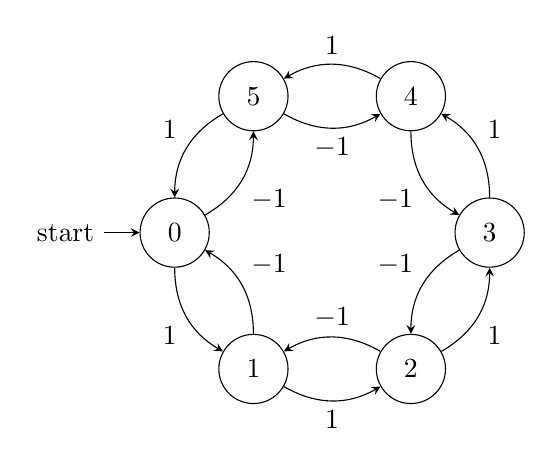
\begin{tikzpicture}[scale=1, transform shape,->,>=stealth]
  \node[state, initial] at ({-2*cos(deg(0*pi/3))},{-2*sin(deg(0*pi/3))}) (q1) {$0$};
  \node[state] at ({-2*cos(deg(1*pi/3))},{-2*sin(deg(1*pi/3))}) (q2) {$1$};
  \node[state] at ({-2*cos(deg(2*pi/3))},{-2*sin(deg(2*pi/3))}) (q3) {$2$};
  \node[state] at ({-2*cos(deg(3*pi/3))},{-2*sin(deg(3*pi/3))}) (q4) {$3$};
  \node[state] at ({-2*cos(deg(4*pi/3))},{-2*sin(deg(4*pi/3))}) (q5) {$4$};
  \node[state] at ({-2*cos(deg(5*pi/3))},{-2*sin(deg(5*pi/3))}) (q6) {$5$};
  \draw (q1) edge[bend right, below left] node{$1$} (q2)
        (q2) edge[bend right, below] node{$1$} (q3)
        (q3) edge[bend right, below right] node{$1$} (q4)
        (q4) edge[bend right, above right] node{$1$} (q5)
        (q5) edge[bend right, above] node{$1$} (q6)
        (q6) edge[bend right, above left] node{$1$} (q1);
  \draw (q2) edge[bend right, above right] node{$-1$} (q1)
        (q3) edge[bend right, above] node{$-1$} (q2)
        (q4) edge[bend right, above left] node{$-1$} (q3)
        (q5) edge[bend right, below left] node{$-1$} (q4)
        (q6) edge[bend right, below] node{$-1$} (q5)
        (q1) edge[bend right, below right] node{$-1$} (q6);
\end{tikzpicture}
\end{center}
\caption{Automata representing the group $\Z/6\Z=\left<1\right>$, this is
  denoted as
  $A_0=\left(\left\{1\right\},\left\{0,1,2,3,4,5\right\},\phi,\psi,0\right)$,
  where $\phi(q,d)=q+d$, and $\psi(q,d)=d$.}\label{fig:z6z_auto}
\end{figure}

Consider the automota represented in Figure \ref{fig:z6z_auto}. Applying this
automata to the \textit{word} of \texttt{11-111-1-1}, we can see how this
automata converts this sequence of generator operations into an element of the
group.

\begin{center}
  \begin{tabular}{r|l}
    State & Word\\
    \hline\hline
    0 & \texttt{11-111-1-1}\\
    1 & \texttt{1-111-1-1}\\
    2 & \texttt{-111-1-1}\\
    1 & \texttt{11-1-1}\\
    2 & \texttt{1-1-1}\\
    3 & \texttt{-1-1}\\
    2 & \texttt{-1}\\
    1 & \texttt{}\\
  \end{tabular}
\end{center}

Thus this word represents the element $1$ in the group. This same process can
be done for any sequence of generators, and as long as the sequence of
generators is finite, then using an automota group can be used to algorithmicly
determine when two different representations represent the same element of the
group.

\section{The Word Problem}%
\label{sec:the_word_problem}

The word problem in relation to groups asks if there is some algorithmic method
to decide whether an element given in terms of a product of generators is
equivalent to another product of generators. It is not possible to solve the
word problem in general, this means that given two products of generators one
cannot tell if they represent the same element.

\end{document}
